%%%%%%%%%%%%%%%%%%%%%%%%%%%%%%%%%%%%%%%%%%%%%%%%%%%%%%%%%%%%%%%%%%%%%%%%%%%%%%%%%%
\begin{frame}[fragile]\frametitle{}
\begin{center}
{\Large Introduction to Yoga and Yogic Practices}
\end{center}
\end{frame}

%%%%%%%%%%%%%%%%%%%%%%%%%%%%%%%%%%%%%%%%%%%%%%%%%%%%%%%%%%%
\begin{frame}[fragile]\frametitle{Syllabus}

\begin{itemize}
\item 1.1  Yoga : Etymology, definitions, aim, objectives and misconceptions. 
\item 1.2  Yoga : Its origin, history and development. 
\item 1.3  Guiding principles to be followed by Yoga practitioners.  
\item 1.4  Principles of Yoga (Triguna, Antahkarana-chatustaya, Tri-Sharira/ Panchakosha). 
\item 1.5  Introduction to major schools of Yoga (Jnana, Bhakti, Karma, Patanjali, Hatha). 
\item 1.6  Introduction to Yoga practices for health and well being. 
\item 1.7  Introduction to Shatkarma: meaning, purpose and their significance in Yoga Sadhana. 
\item 1.8  Introduction to Yogic  Sukshma Vyayama,  Sthula Vyayama and Surya Namaskara.  
\item 1.9  Introduction to Yogasana: meaning, principles, and their health benefits. 
\item 1.10  Introduction to Pranayama and Dhyana and their health benefits. 
\end{itemize}
	  
\end{frame}

%%%%%%%%%%%%%%%%%%%%%%%%%%%%%%%%%%%%%%%%%%%%%%%%%%%%%%%%%%%%%%%%%%%%%%%%%%%%%%%%%%
\begin{frame}[fragile]\frametitle{}
\begin{center}
{\Large Background Terms}
\end{center}
\end{frame}

%%%%%%%%%%%%%%%%%%%%%%%%%%%%%%%%%%%%%%%%%%%%%%%%%%%%%%%%%%%
\begin{frame}[fragile]\frametitle{Understanding Key Concepts}
      \begin{itemize}
        \item \textbf{brahman ब्रह्मन् }: Absolute reality, infinite, uncaused, eternal, source of being, intelligence, and bliss (sat chit anand सत्-चित्-आनन्द).
        \item \textbf{maaya माया}: Creative and illusory power of ब्रह्मन्, cosmic illusion, ब्रह्मन् as the unaffected upholder of creation.
        \item \textbf{atman आत्मन्}: Absolute reality in the individual, one with ब्रह्मन्, unchanging, refers to the Absolute within.
        \item \textbf{upaadhi उपाधि}: Limiting adjunct, false identification creating an illusion of limitation, body and mind.
        \item \textbf{avidya अविद्या}: Primordial ignorance, wrong identification with उपधि.
        \item \textbf{jeev जीव}: Apparent individual soul, self identifying with उपधि, suffers due to perceived limitations, reborn until realizing true nature (आत्मन्).
        \item \textbf{ishwar ईश्वर}: ब्रह्मन् with माया, personal God, endowed with omniscience, omnipresence, and unlimited power, creator, preserver, destroyer.
        \item \textbf{purush पुरुष}: Absolute consciousness, as described in sankhya-yoga साङ्ख्य -योग .
        \item \textbf{prakruti प्रकृति}: Material cause of creation, three गुण  in balance, potential creation, माया.
      \end{itemize}
	  
\textbf{Summary}: माया manifests as अविद्या , leading to identification with उपाधि. जीव suffers due to this false identification until realizing आत्मन्.	  
\end{frame}



%%%%%%%%%%%%%%%%%%%%%%%%%%%%%%%%%%%%%%%%%%%%%%%%%%%%%%%%%%%%%%%%%%%%%%%%%%%%%%%%%%
\begin{frame}[fragile]\frametitle{}
\begin{center}
{\Large 1.1 Yoga : Etymology, definitions, aim, objectives and misconceptions}
\end{center}
\end{frame}

%%%%%%%%%%%%%%%%%%%%%%%%%%%%%%%%%%%%%%%%%%%%%%%%%%%%%%%%%%%
\begin{frame}[fragile]\frametitle{Etymology of Yoga}

      \begin{itemize}
		\item Etymology: study of the origin of word. शब्द व्युत्पत्ती शास्त्र 
		\item Sanskrit word \textit{योग} (Yoga), root \textit{युज्} (Yuj) meaning “to join” or “to unite”.(युज संयोग)
		\item Union of  जीवात्मा  jeevatma  (individual  self) with with the परमात्मा paramatma (the universal self). In other words, yoga is the union of the “apparent man” identified with  body, mind and senses with the “real man” who is 
free from all sorts of worldly limitations.
\item Union of ``Body, Mind and Spirit'' as the purpose of Yoga is to attain spiritual perfection through the control 
of the body, senses and mind
		\item According to Panini, verbal root युज  yuj has three 
connotations: to union (युजिर योगे), to focus (युज समाधौ, used in Patanjali's Yogasutra and by Vyasa), to control (युज सैयमने , )
		\item Yoga is 'end/goal' (साध्य ) as well as 'means/tools'(साधना)
		% \item Ancient practice with origins in the Vedic texts and Upanishads.
		% \item Evolved through various philosophies and traditions over centuries.
	  \end{itemize}

\end{frame}

%%%%%%%%%%%%%%%%%%%%%%%%%%%%%%%%%%%%%%%%%%%%%%%%%%%%%%%%%%%
\begin{frame}[fragile]\frametitle{Definitions of Yoga}
      \begin{itemize}
        \item \textbf{पतञ्जलि  योगसूत्र  Patanjali Yoga Sutras}:      योगश्चित्तवृत्तिनिरोधः || १:२ || To block the patterns of consciousness is Yoga.
        \item \textbf{Yoga Vasishtha योगवशिष्ठ }:          मनः प्रशमनोपायः योग इत्यभिधीयते | Yoga is called a skillful trick to calm down the mind.
        \item \textbf{भगवद्गीता  Bhagavad Gita}:         
		      \begin{itemize}
				\item  योगस्थः कुरु कर्माणि सङ्गं त्यक्त्वा धनञ्जय |   सिद्ध्यसिद्ध्योः समो भूत्वा \textbf{समत्वं योग उच्यते }|| २:४८ || O Dananjaya, perform action being steadfast in Yoga, abandoning attachment and remaining equanimous in success and failure. Yoga is the equanimity of mind.
				\item बुद्धियुक्तो जहातीह उभे सुकृतदुष्कृते |      तस्माद्योगाय युज्यस्व \textbf{योगः कर्मसु कौशलम् }|| २:५० || Endowed with wisdom of equanimity, cast off in this life both good and bad deeds. Thus, dedicate yourself to Yoga. Skill in Action is Yoga.
				\item युक्ताहारविहारस्य युक्तचेष्टस्य कर्मसु |युक्तस्वप्नावबोधस्य \textbf{योगो भवति दु:खहा }||६ .१ ७ || Those who are temperate in eating and recreation, balanced in work, and regulated in sleep, can mitigate all sorrows by practicing Yog.
				\end{itemize}
		\item \textbf{Kathopanishad कठोपनिषद २/५/४}: तां योगामिती मन्यतें स्थिरमिन्द्रिय धारणं The state unperturbed when the senses are imprisoned in the mind, of this they say, it is Yoga.
      \end{itemize}
\end{frame}

% %%%%%%%%%%%%%%%%%%%%%%%%%%%%%%%%%%%%%%%%%%%%%%%%%%%%%%%%%%%
% \begin{frame}[fragile]\frametitle{Definitions of Yoga}
      % \begin{center}
        % 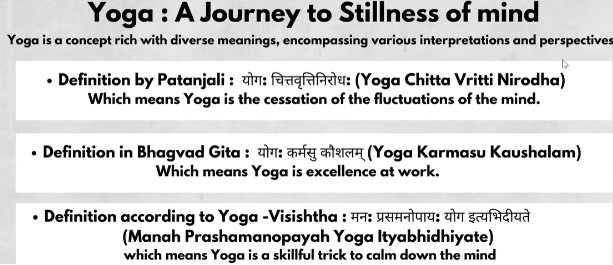
\includegraphics[width=\linewidth,keepaspectratio]{ycb1_definitions}

		% {\tiny (Ref: Param Yoga)}		
        % \end{center}

% \end{frame}

% %%%%%%%%%%%%%%%%%%%%%%%%%%%%%%%%%%%%%%%%%%%%%%%%%%%%%%%%%%%
% \begin{frame}[fragile]\frametitle{Meaning and concepts of Yoga}
% Four Ashrams of Vedic Life: Based on karma कर्म and dharma धर्म, Vedic life was divided into four ashrams: 

          % \begin{itemize}
            % \item \textbf{The First Ashrama - brahmacharya } - "ब्रह्मचर्य" or the Student Stage
            % \item \textbf{The Second Ashrama - gruhastha } - "गृहस्थ" or the Householder Stage
            % \item \textbf{The Third Ashrama - vaanaprastha } - "वानप्रस्थ" or the Hermit Stage
            % \item \textbf{The Fourth Ashrama - sanyas } - "संन्यास" or the Wandering Ascetic Stage
          % \end{itemize}
		  
% Purusharthas ( पुरुषार्थ )literally means ``aims of man'' or ``what men live for''. It is the prescription for the right way of living, recognizing various inherent urges and satisfying them for a meaningful life.
          
          % \begin{itemize}
            % \item \textbf{dharma धर्म}: Righteousness
            % \item \textbf{aarth अर्थ}: Wealth or material means
            % \item \textbf{kaam काम}: Satisfaction of sensual desires
            % \item \textbf{moksh मोक्ष}: Freedom or spiritual liberation
          % \end{itemize}
% \end{frame}

% %%%%%%%%%%%%%%%%%%%%%%%%%%%%%%%%%%%%%%%%%%%%%%%%%%%%%%%%%%%
% \begin{frame}[fragile]\frametitle{The Gurus and Gurukul System}
      % \begin{itemize}
        % \item {\textit “To light the candle one needs another burning candle; in the same way, those who are unenlightened need the help of an illumined Guru.”} - Swami Sivananda
          
          % \item The word Guru:  गु meaning "Darkness" and रु meaning "to destroy". 
		  % \item A Guru is a spiritually enlightened being that dispels the darkness of ignorance and lifts the veil of माया (illusion), rendering the disciple free from the cycle of death and birth.
          
          
          % % The journey stops with the finding of the Guru. The Guru is the gateway to the infinite, guiding the disciple towards the personal realization of the eternal truth.
          
          
          % % The love between Guru and disciple transcends all human relationships. It is through this relationship that the disciple's potential is given shape and direction, working towards the divine plan.
          
        % \item \textbf{The Gurukul System in India}: Gurukul गुरुकुल translates to "the home (family) of the preceptor." 
		% \item The Guru गुरु lives with his family and disciples. Students come to be part of the Guru's family, learning Vedas, Sanskrit, fine arts, administration, and other skills and etiquette.
          
          
          % % Gurukuls were in forests or by riversides. The first 25 years of life, as ब्रह्मचर्य (a celibate student), were spent acquiring training for serving society and personal emancipation.
          
          
          % % Life in Gurukul involved rigorous तपस (austerities) to prepare for life's hardships, instilling habits like hard work, enthusiasm, and selfless service. Students performed duties like fetching water, cleaning, and gathering twigs, while practicing meditation and Yoga.
          
          
          % % Classes were held under shady banyan trees or in thatched huts. Education was generally free, but the Guru received दक्षिणा (fee) from disciples.
          
      % \end{itemize}
% \end{frame}


%%%%%%%%%%%%%%%%%%%%%%%%%%%%%%%%%%%%%%%%%%%%%%%%%%%%%%%%%%%
\begin{frame}[fragile]\frametitle{Aims/Objectives of Yoga}

      \begin{itemize}
		\item आहार  Aahar, व्यवहार  Vyavahar, आचार  Achar, विचार  Vichar, and विहार  Vihar are pillars of yoga that are said to help you live a healthy and happy life.
		\item To cultivate \textit{Discipline} and \textit{Self-Control}.
		\item To improve \textit{Mental Focus} and \textit{Concentration}.
		\item To enhance \textit{Emotional Stability} and \textit{Resilience}.
		\item To promote \textit{Physical Fitness} and \textit{Posture}.
		\item To achieve \textit{Holistic Well-Being} and \textit{Harmonious Living}.
		% \item लक्ष्य : स्व चे आकलन. आत्मा ते परमात्मा प्रवास 
		% \item उद्देश : सर्वांगीण विकास, सामंजस्य स्थापना. मन बुद्धी व चरित्र यांना शुद्ध बनवणे		
		\item लक्ष्य: स्वयं का आकलन, आत्मा से परमात्मा की यात्रा।
		\item उद्देश्य: सर्वांगीण विकास, सामंजस्य की स्थापना। मन, बुद्धि और चरित्र को शुद्ध बनाना।
	  \end{itemize}

\end{frame}

%%%%%%%%%%%%%%%%%%%%%%%%%%%%%%%%%%%%%%%%%%%%%%%%%%%%%%%%%%%
\begin{frame}[fragile]\frametitle{Misconceptions about Yoga}

      \begin{itemize}
		\item Yoga is only about physical postures (\textit{aasan आसन }).
		\item Yoga is a religion.
		\item Yoga requires flexibility.
		\item Yoga is just about relaxation.
		\item Yoga is a practice for only young people.
		% \item  धर्म : फक्त हिंदूंसाठी नाही. वैश्विक. 
		% \item  व्यायाम: फक्त शारीरिक नाही तर मानसिक आणि आध्यत्मिक . 
		% \item  चमत्कार/प्रदर्शन/सिद्धी प्राप्ती 
		% \item  तरुणांसाठीच नाही  तर सर्वांसाठी 
		\item  धर्म: केवल हिंदुओं के लिए नहीं, बल्कि सार्वभौमिक।
		\item  व्यायाम: केवल शारीरिक नहीं, बल्कि मानसिक और आध्यात्मिक भी।
		\item  चमत्कार/प्रदर्शन/सिद्धि प्राप्ति।
		\item  युवाओं के लिए ही नहीं, बल्कि सभी के लिए।		
	  \end{itemize}

\end{frame}


%%%%%%%%%%%%%%%%%%%%%%%%%%%%%%%%%%%%%%%%%%%%%%%%%%%%%%%%%%%%%%%%%%%%%%%%%%%%%%%%%%
\begin{frame}[fragile]\frametitle{}
\begin{center}
{\Large 1.2 Yoga : Its origin, history and development}
\end{center}
\end{frame}


%%%%%%%%%%%%%%%%%%%%%%%%%%%%%%%%%%%%%%%%%%%%%%%%%%%%%%%%%%%
\begin{frame}[fragile]\frametitle{Origin of Yoga}

      \begin{itemize}
		\item Originated in ancient India around 5000 BCE.
		\item First mentions in the \textit{ऋग्वेद  Rigveda} and \textit{यजुर्वेद  Yajurveda}.
		\item One of the षटदर्शन  6 Indian philosophical systems (दर्शन ) like \textit{सांख्य  Samkhya} and \textit{वेदान्त  Vedanta}.
        % \item \textbf{Ancient Roots}: 
          
          % Yoga originated in ancient India. The origin of Yoga is traced to the वेद (Vedas). It is difficult to ascertain a fixed time period for the origin of these ancient texts due to differing historical accounts.
          
        % \item \textbf{Ancient Tradition}: 
          
          % The system of Yoga is an ancient tradition having its origin in India. The practice of Yoga is believed to have started at the very dawn of civilization.
          
        \item \textbf{Yogic Lore}: 
          
          In the Yogic lore, Lord Shiva is considered to be the first yogi or आदियोगी (Adiyogi), and the first Guru or आदि गुरु (Adi Guru).
          		
		% \item उत्पत्ती: हजारो वर्षांपूर्वी, भारतात. शिव हे आदी योगी आणि गुरु. सप्तर्षींद्वारा प्रसार. 
		% \item प्राचीन पुरातत्व अवशेषांवरून सिद्ध होते कि सिंधू हडप्पा संस्कृतीत योग होता, मुद्रा मुर्त्या होत्या. 
		% \item साहित्य: “हिरण्यगर्भ योगस्य वक्ता मान्य:पुरातन:”, वेद , उपनिषद , दर्शन, बौद्ध, जैन परंपरा 
		% \item पतंजली योगसूत्र 		
		\item उत्पत्ति: हजारों वर्ष पहले, भारत में। शिव आदि योगी और गुरु। सप्तर्षियों द्वारा प्रसार।
		\item प्राचीन पुरातत्व अवशेषों से सिद्ध होता है कि सिंधु हड़प्पा संस्कृति में योग था, मुद्राएं और मूर्तियां थीं।
		\item साहित्य: “हिरण्यगर्भ योगस्य वक्ता मान्य: पुरातन:”, वेद, उपनिषद, दर्शन, बौद्ध, जैन परंपरा।
		\item  पतंजलि योगसूत्र।
	  \end{itemize}

\end{frame}

%%%%%%%%%%%%%%%%%%%%%%%%%%%%%%%%%%%%%%%%%%%%%%%%%%%%%%%%%%%
\begin{frame}[fragile]\frametitle{Historical Development of Yoga}

      \begin{itemize}
	    \item \textit{Vedic Period}: मंत्रयोग ,  प्राणयोग , ध्यानयोग  mantra yoga, praan yoga, dhyan yoga. Rigveda.(\textit{1500-500 BCE})
		\item \textit{Pre-Classical Period}:  Upanishads and early Yoga texts  (\textit{500 -200 BCE}).
		\item \textit{Classical Period}: \textit{Yoga Sutras of  पतञ्जलि  Patanjali} and \textit{bhagavadgeeta भगवद्गीता } (\textit{200 BCE - 500 CE}).
		\item \textit{Post-classical/Medieval Period}: Development of \textit{hathayoga हठयोग } and tantric traditions (\textit{500 -1700 CE}). Hathayoga is Tantra yoga after removing some controversial practices.
		\item \textit{Modern Period}: Revival and global dissemination in the 19th and 20th centuries. Major figures: Swami Vivekananda, Sri T. Krishnamacharya, B.K.S. Iyengar. (Post 1700)
		\item \textit{वैदिक: १५०० इ पूर्व - ५०० इ पूर्व }: सूर्यनमस्कार प्राणायाम , वेद, पाणिनी 
		\item \textit{अवधी: ५०० इ पूर्व -  २ ० ०  इ पूर्व }: उपनिषद
		\item \textit{श्रेष्ठ अवधी:  २ ० ०  इ पूर्व - ५००}: पतंजली  योगसूत्र , व्यास भगवद्गीता , महावीर पंचमहाव्रत, बुद्ध अष्टांगिक मार्ग 
		\item \textit{पश्चात : ५०० - १७००}: आदी शंकराचार्य , रामानुजाचार्य , माधवाचार्य, भक्तियोगी (कबीर, तुलसी), हटयोगी (नाथ संप्रदाय)
		\item \textit{आधुनिक : १७०० के बाद}: रमण महर्षी , विवेकानंद, परमहंस योगानंद, टी कृष्णमाचार्य, सत्यानंद सरस्वती 
		
	  \end{itemize}

\end{frame}

%%%%%%%%%%%%%%%%%%%%%%%%%%%%%%%%%%%%%%%%%%%%%%%%%%%%%%%%%%%
\begin{frame}[fragile]\frametitle{History of Yoga}
      \begin{center}
        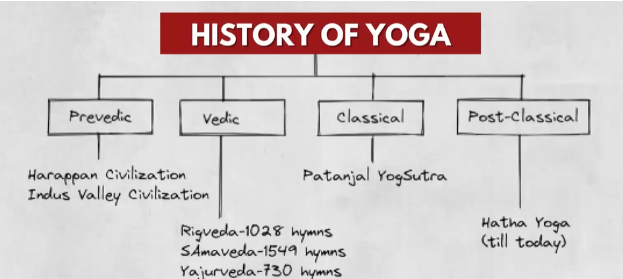
\includegraphics[width=0.7\linewidth,keepaspectratio]{ycb1_history}

        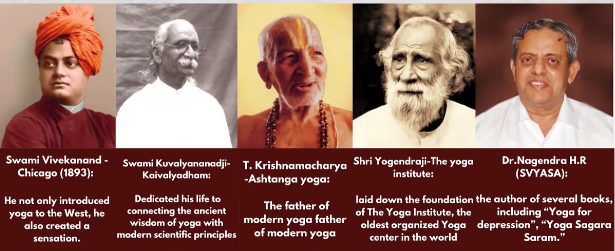
\includegraphics[width=0.7\linewidth,keepaspectratio]{ycb1_teachers}

		{\tiny (Ref: Param Yoga)}		
        \end{center}

\end{frame}

%%%%%%%%%%%%%%%%%%%%%%%%%%%%%%%%%%%%%%%%%%%%%%%%%%%%%%%%%%%
\begin{frame}[fragile]\frametitle{Key Texts and Influences}

      \begin{itemize}
		\item \textit{vaidik वैदिक} - Early ritualistic and philosophical foundations.
		\item \textit{upanishad उपनिषद } - Conceptual framework of Yoga.
		\item \textit{patanjali yogasutra पतंजली योगसूत्र} - Systematization of Yoga philosophy.
		\item \textit{bhagavadgeeta भगवद्गीता} - Integration of Yoga with life and duty.
		\item \textit{hathayoga pradipika हठयोग प्रदीपिका } - Practical techniques and practices.
		\item \textit{भारतीय दर्शन} :
			\begin{itemize}
			% \item \textit{आस्तिक (वेद मानणारे)}: न्याय (गौतम), वैशेषिक (कणाद), सांख्य (कपिल), मीमांसा (जैमिनी), योग(पतंजली), वेदांत (बादरायण)
			% \item \textit{नास्तिक} : जैन (महावीर), बौद्ध , चार्वाक (बृहस्पती)
			\item \textit{आस्तिक (वेद मानने वाले)}: न्याय (गौतम), वैशेषिक (कणाद), सांख्य (कपिल), मीमांसा (जैमिनी), योग (पतंजलि), वेदांत (बादरायण)।
			\item \textit{नास्तिक}: जैन (महावीर), बौद्ध, चार्वाक (बृहस्पति)।
		    \end{itemize}
	    \item Samkhya philosophy teaches dualism through Purusha (consciousness) and Prakriti (matter) as two eternal principles.
	    \item All matter is composed of the three gunas: sattva, rajas, and tamas.
	    \item The ultimate goal, Kaivalya (liberation), is achieved by distinguishing Purusha from Prakriti to end suffering (sources: adhyatmic, adhibhautic, and adhidaivic griefs).
	  \end{itemize}

\end{frame}

%%%%%%%%%%%%%%%%%%%%%%%%%%%%%%%%%%%%%%%%%%%%%%%%%%%%%%%%%%%
\begin{frame}[fragile]\frametitle{Evolution of Yoga Practices}

      \begin{itemize}
		\item Early practices focused on meditation and asceticism.
		\item Development of physical postures (\textit{aasan आसन }) in the medieval period.
		\item Integration of breath control (\textit{pranayam प्राणायाम }) and energy channels (\textit{naadi नाडी }).
		\item Emergence of different styles: \textit{hath हठ}, \textit{kundalini कुण्डलिनि }, \textit{raajyoga राज योग}, and \textit{karma yoga कर्म  योग}.
		\item Contemporary practices: \textit{विन्यास }, \textit{अष्टान्ग }, and \textit{Power Yoga}.
		% \item  सूक्ष्म व्यायाम: हलके, योगाभ्यासाच्या आधी. स्वामी धीरेंद्र ब्रह्मचारी (गुरु: कार्तिकेय महाराज) . शरीर लवचिक व तयार होते. 
		% \item स्थूल व्यायाम: सर्व शरीराचा, गतीचा, शक्तीचा संचार . 
		\item सूक्ष्म व्यायाम: हल्के, योगाभ्यास से पहले। स्वामी धीरेंद्र ब्रह्मचारी (गुरु: कार्तिकेय महाराज)। शरीर लचीला और तैयार होता है।
		\item सस्थूल व्यायाम: पूरे शरीर का, गति और शक्ति का संचार।
	  \end{itemize}

\end{frame}



%%%%%%%%%%%%%%%%%%%%%%%%%%%%%%%%%%%%%%%%%%%%%%%%%%%%%%%%%%%%%%%%%%%%%%%%%%%%%%%%%%
\begin{frame}[fragile]\frametitle{}
\begin{center}
{\Large 1.3 Guiding principles to be followed by Yoga practitioners}
\end{center}
\end{frame}

%%%%%%%%%%%%%%%%%%%%%%%%%%%%%%%%%%%%%%%%%%%%%%%%%%%%%%%%%%%%%%%%%%%%%%%%%%%%%%%%%%
\begin{frame}[fragile]\frametitle{Guiding Principles for Yoga Teachers Practitioners}

\begin{itemize}
    \item \textbf{Preparation:} Ensure a clean, well-ventilated space free from distractions. For online classes, check internet connectivity, settings etc.
    \item \textbf{Diet:} Practice on an empty or light stomach to optimize \textit{प्राण शक्ती Prana Shakti} (vital force) for healing and repair.
    \item \textbf{Starting the Class:} Begin with a prayer or mantra. 
	% If the practitioner is uncomfortable with Sanskrit chanting, offer alternatives like affirmations, or allow them to say their own prayer silently.
    \item \textbf{Touch and Posture Correction:} Always seek permission before touching practitioners for posture correction, especially in Western contexts. % Use non-verbal cues (e.g., turning palms upside) to indicate discomfort.
    \item \textbf{Verbal Cues:} Provide clear, precise instructions, particularly in online classes. Include reminders for breathing, alignment, and maintaining connection with the stretch.
    \item \textbf{Post-Practice:} Avoid drinking water, showering, or eating immediately after practice to allow the body’s heat to dissipate naturally. A gap of 40 minutes to 1 hour is recommended.
    \item \textbf{Feedback:} Keep time at the end of the class for feedback and open conversation to improve future sessions.
\end{itemize}

\end{frame}

%%%%%%%%%%%%%%%%%%%%%%%%%%%%%%%%%%%%%%%%%%%%%%%%%%%%%%%%%%%
\begin{frame}[fragile]\frametitle{Guiding Principles for Yoga Practitioners}

By Swami Vishnudevananda

    \begin{itemize}
        \item \textbf{Proper Exercise - aasan आसन}
            
            % आसन (Asana) develops the body, broadens mental faculties, and spiritual capacities. Unlike violent physical exercises, yoga postures focus on maintaining the spine’s flexibility and strength.
            
        \item \textbf{Proper Breathing - pranayam प्राणायाम}
            
            % प्राणायाम (Pranayama) involves controlling प्राण (Prana) to achieve control over the mind. Proper breathing increases lung capacity and vitality.
            
        \item \textbf{Proper Relaxation - shavasan  शवासन }
            
            % सवासन (Savasana) is the corpse pose, a state of physical, mental, and spiritual relaxation that recharges and balances the body and mind.
            
        \item \textbf{Proper Diet - Vegetarian}
            
            % A Yogic diet consists of pure, simple, natural foods that promote health. Vegetarian meals aid digestion and provide balanced nutrition.
            
        \item \textbf{Positive Thinking and Meditation - vedant  वेदान्त  and dhyan ध्यान }
            
            % ध्यान (Dhyana) is the practice of meditation that focuses the mind internally on the self, leading to lasting happiness and peace.
            
    \end{itemize}
\end{frame}


%%%%%%%%%%%%%%%%%%%%%%%%%%%%%%%%%%%%%%%%%%%%%%%%%%%%%%%%%%%%%%%%%%%%%%%%%%%%%%%%%%
\begin{frame}[fragile]\frametitle{}
\begin{center}
{\Large 1.4 Principles of Yoga (त्रिगुण Triguna, अन्त:करण -चतुस्तय Antahkarana-chatustaya,त्रिशरिर  TriSharira/  पञ्चकोष Panchakosha)}
\end{center}
\end{frame}

%%%%%%%%%%%%%%%%%%%%%%%%%%%%%%%%%%%%%%%%%%%%%%%%%%%%%%%%%%%
\begin{frame}[fragile]\frametitle{त्रिगुण  (Three गुण )}

      \begin{itemize}
		\item \textit{sattva सत्व } - Quality of purity, clarity, and harmony.
		\item \textit{rajas रजस } - Quality of activity, movement, and restlessness.
		\item \textit{tamas तमस } - Quality of inertia, darkness, and ignorance.
		\item Balance of गुण  affects mental and emotional states.
		\item Goal: Cultivate \textit{सत्व} for spiritual growth and peace.
	  \end{itemize}

\end{frame}

%%%%%%%%%%%%%%%%%%%%%%%%%%%%%%%%%%%%%%%%%%%%%%%%%%%%%%%%%%%
\begin{frame}[fragile]\frametitle{अन्त:करण -चतुस्तय  (Four Aspects of the Inner Instrument)}

      \begin{itemize}
		\item \textit{manas मनस } (Mind) - Handles thoughts and sensory perceptions.
		\item \textit{buddhi बुद्धि } (Intellect) - Functions as the decision-making faculty.
		\item \textit{ahamkaar अहंकार } (Ego) - Sense of individuality and self-identity.
		\item \textit{chitta चित्त } (Memory) - Stores past experiences and impressions.
		\item Harmonizing these aspects aids in mental clarity and self-awareness.
	  \end{itemize}

\end{frame}

%%%%%%%%%%%%%%%%%%%%%%%%%%%%%%%%%%%%%%%%%%%%%%%%%%%%%%%%%%%
\begin{frame}[fragile]\frametitle{त्रिशरिर  Tri-Sharira (Three Bodies)}

      \begin{itemize}
		\item \textit{sthula sharir स्थूल  शरीर } (Gross Body) - Physical body made of elements.
		\item \textit{sukshma sharir सूक्ष्म  शरीर } (Subtle Body) - Includes mind, intellect, and ego.
		\item \textit{kaaran sharir कारण  शरीर } (Causal Body) - The essence of individuality and karma.
		\item Understanding these bodies aids in holistic self-realization.
		\item Goal: Achieve harmony among all three bodies for spiritual growth.
	  \end{itemize}

\end{frame}

%%%%%%%%%%%%%%%%%%%%%%%%%%%%%%%%%%%%%%%%%%%%%%%%%%%%%%%%%%%
\begin{frame}[fragile]\frametitle{पञ्चकोष   (Five Sheaths)}

      \begin{itemize}
		\item \textit{अन्नमय  annamay कोष  kosh} (Food Sheath) - Physical body nourished by food.
		\item \textit{प्राणमय  praanamay  कोष  kosh} (Vital Air Sheath) - Energy body responsible for life force.
		\item \textit{मनोमय  manomay कोष kosh } (Mental Sheath) - Mind and emotional body.
		\item \textit{विज्ञानमय Vijnanamaya कोष  kosh} (Wisdom Sheath) - Intellect and discernment.
		\item \textit{आनन्दमय Anandamaya कोष  kosh} (Bliss Sheath) - True self, source of bliss and consciousness.
		\item Goal: Transcend the sheaths to realize the true self.
	  \end{itemize}

      \begin{center}
        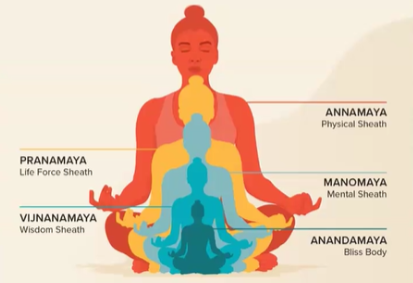
\includegraphics[width=0.4\linewidth,keepaspectratio]{ycb1_kosha}

		{\tiny (Ref: Param Yoga)}		
        \end{center}
\end{frame}

%%%%%%%%%%%%%%%%%%%%%%%%%%%%%%%%%%%%%%%%%%%%%%%%%%%%%%%%%%%
\begin{frame}[fragile]\frametitle{पञ्च  महाभूत  Pancha Maha Bhuta: Five Elements}


    \begin{itemize}
        \item \textbf{Akasha आकाश  (Space/Ether)}
        \item \textbf{Vayu वायु  (Air)}
        \item \textbf{Agni अग्नि (Fire)}
        \item \textbf{Jala जल (Water)}
        \item \textbf{Prithvi पृथ्वी (Earth)}
    \end{itemize}
	
    \textbf{Elemental Sequence:}
	
    \begin{itemize}
        \item From आकाश (Akasha) comes वायु (Vayu)
        \item From वायु (Vayu) comes अग्नि (Agni)
        \item From अग्नि (Agni) comes जल (Jala)
        \item From जल (Jala) comes पृथ्वी (Prithvi)
    \end{itemize}
	
\end{frame}

%%%%%%%%%%%%%%%%%%%%%%%%%%%%%%%%%%%%%%%%%%%%%%%%%%%%%%%%%%%
\begin{frame}[fragile]\frametitle{पञ्च  महाभूत   Pancha Maha Bhuta: Five Elements}

    \textbf{Physical Properties and Functions:}
	
	
        \begin{tabular}{|p{0.21\linewidth}|p{0.1\linewidth}|p{0.1\linewidth}|p{0.1\linewidth}|p{0.1\linewidth}|p{0.1\linewidth}|}
% \begin{tabular}{|l|l|l|l|l|l|}
    \hline
    \textbf{Element} & \textbf{Space/Ether} & \textbf{Air} & \textbf{Fire} & \textbf{Water} & \textbf{Earth} \\
    \hline
    \textbf{Attributes} & Light, Minute, Quick, Clear, Soft & Light, Dry, Rough, Mobile, Cold, Minute, Clear & Dry, Hot, Sharp, Light, Rough, Minute, Clear & Heavy, Moist, Fluid, Slimy, Cold, Thick, Soft & Heavy, Rough, Solid, Massive, Firm, Hard \\
    \hline
    \textbf{Role in the Body} & Body cavities & Movement, pulsation, conduction & Whole body metabolism & All adhesions, joints & Body organs, mass, inertia \\
    \hline
    \end{tabular}

\end{frame}


%%%%%%%%%%%%%%%%%%%%%%%%%%%%%%%%%%%%%%%%%%%%%%%%%%%%%%%%%%%
\begin{frame}[fragile]\frametitle{तन्मात्र Tanmatras and Sense Organs}
    \textbf{तन्मात्र Tanmatras: Fundamental/seed Elements}
	
	
    \begin{tabular}{|l|l|l|}
    \hline
    \textbf{Element} & \textbf{Sanskrit Word} & \textbf{English Translation} \\
    \hline
    \textbf{Space/Ether} & शब्द (Shabda) & Sound \\
    \hline
    \textbf{Air} & स्पर्श (Sparsha) & Touch \\
    \hline
    \textbf{Fire} & रूप (Rupa) & Shape/Visual/Light \\
    \hline
    \textbf{Water} & रस (Rasa) & Taste \\
    \hline
    \textbf{Earth} & गन्ध (Gandha) & Smell \\
    \hline
    \end{tabular}


    \textbf{पञ्च  ज्ञानेन्द्रिय  Pancha Jnanedriya: Five Sense Organs}
	
    \begin{tabular}{|l|l|}
    \hline
    \textbf{Element} & \textbf{Sense Organ} \\
    \hline
    \textbf{Space/Ether} & Ears \\
    \hline
    \textbf{Air} & Skin \\
    \hline
    \textbf{Fire} & Eyes \\
    \hline
    \textbf{Water} & Tongue \\
    \hline
    \textbf{Earth} & Nose \\
    \hline
    \end{tabular}
\end{frame}

%%%%%%%%%%%%%%%%%%%%%%%%%%%%%%%%%%%%%%%%%%%%%%%%%%%%%%%%%%%
\begin{frame}[fragile]\frametitle{पञ्च कर्मेन्द्रिय Pancha Karmendriya: Five Action Organs}
    \begin{tabular}{|l|l|l|}
    \hline
    \textbf{Element} & \textbf{Action Organ} & \textbf{Function} \\
    \hline
    \textbf{Space/Ether} & Tongue & Speech \\
    \hline
    \textbf{Air} & Hand & Receiving and Holding \\
    \hline
    \textbf{Fire} & Feet & Movement \\
    \hline
    \textbf{Water} & Genitals & Reproduction \\
    \hline
    \textbf{Earth} & Anus & Discharging the waste \\
    \hline
    \end{tabular}
\end{frame}

%%%%%%%%%%%%%%%%%%%%%%%%%%%%%%%%%%%%%%%%%%%%%%%%%%%%%%%%%%%
\begin{frame}[fragile]\frametitle{सप्त धातु  Sapta Dhatu: Seven Tissues}
    \begin{itemize}
        \item \textbf{रस  Rasa} - Plasma
        \item \textbf{रक्त  Rakta} - Blood
        \item \textbf{मांस  Mamsa} - Muscle
        \item \textbf{मेद  Meda} - Adipose
        \item \textbf{अस्थि Asthi} - Bone
        \item \textbf{मज्जा Majja} - Bone Marrow
        \item \textbf{शुक्र Shukra} - Reproductive Tissues
    \end{itemize}
    \vspace{0.5cm}
    \textbf{Function:} 
    
    धातु (Dhatu) sustains and maintains the body, with each Dhatu providing nourishment to the next.
    
\end{frame}

%%%%%%%%%%%%%%%%%%%%%%%%%%%%%%%%%%%%%%%%%%%%%%%%%%%%%%%%%%%
\begin{frame}[fragile]\frametitle{त्रिदोष  Tri Doshas: Three Constitutions}
    \begin{tabular}{|l|l|}
    \hline
    \textbf{दोष Dosha} & \textbf{Properties} \\
    \hline
    \textbf{वात  Vata} & Dry, Light, Cold, Rough, Minute, Unsteady \\
    \hline
    \textbf{पित्त Pitta} & Unctuous, Hot, Sharp, Light, Bad Smell, Quick in movement, Liquid \\
    \hline
    \textbf{कफ  Kapha} & Unctuous, Cold, Massive, Sluggish, Slippery, Soft, Steady \\
    \hline
    \end{tabular}
    \vspace{0.5cm}
    \textbf{दोष Dosha Meaning:}
    
    दोष (Dosha) means 'that which vitiates' and can be seen as a fault or imbalance in the cosmic rhythm.
    
\end{frame}

%%%%%%%%%%%%%%%%%%%%%%%%%%%%%%%%%%%%%%%%%%%%%%%%%%%%%%%%%%
\begin{frame}[fragile]\frametitle{पञ्च  प्राण  Pancha Prana: Five Pranas in the Body}
    \begin{itemize}
        \item \textbf{प्राण Prana } - From the head down to the navel
        \item \textbf{अपान Apana} - From the navel down to the मूलाधार  चक्र  Muladhara chakra
        \item \textbf{उदान Udana} - From the navel to the head
        \item \textbf{समान Samana} - In the navel region
        \item \textbf{व्यान Vyana} - Throughout the body
    \end{itemize}
    \vspace{0.5cm}
    \textbf{उपप्राण Upapranas:}
    \begin{itemize}
        \item \textbf{नाग  Naga} - Hiccoughs, Burps
        \item \textbf{कुर्म  Kurma} - Blinking of the eyes
        \item \textbf{कृकल Krikal} - Hunger, Thirst, Sneezing, Coughing
        \item \textbf{देवदत्त Devadatta} - Yawning, Drowsiness
        \item \textbf{धनञ्जय Dhananjaya} - After death lingering
    \end{itemize}
\end{frame}

%%%%%%%%%%%%%%%%%%%%%%%%%%%%%%%%%%%%%%%%%%%%%%%%%%%%%%%%%%
\begin{frame}[fragile]\frametitle{प्राण Pranas}
        \begin{center}
        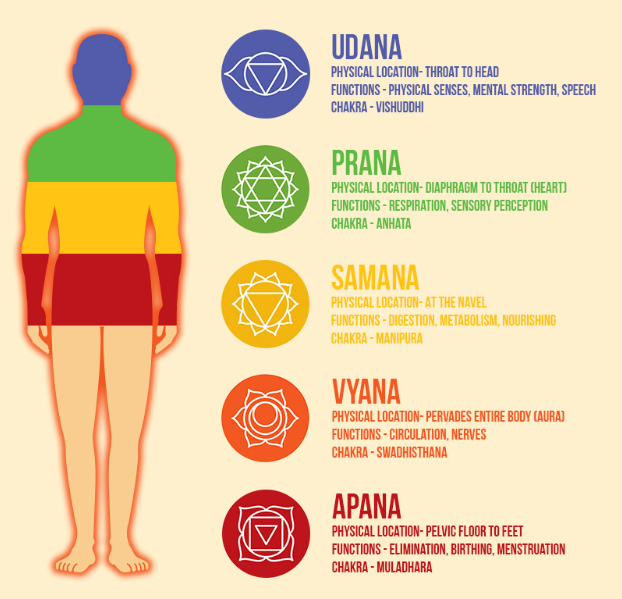
\includegraphics[width=0.6\linewidth,keepaspectratio]{ycb1_pranas}
				
		{\tiny (Ref: Raja Yoga Rishikesh)}	 
        \end{center}	

\end{frame}
%%%%%%%%%%%%%%%%%%%%%%%%%%%%%%%%%%%%%%%%%%%%%%%%%%%%%%%%%%
\begin{frame}[fragile]\frametitle{चक्र  Chakras}
        \begin{center}
        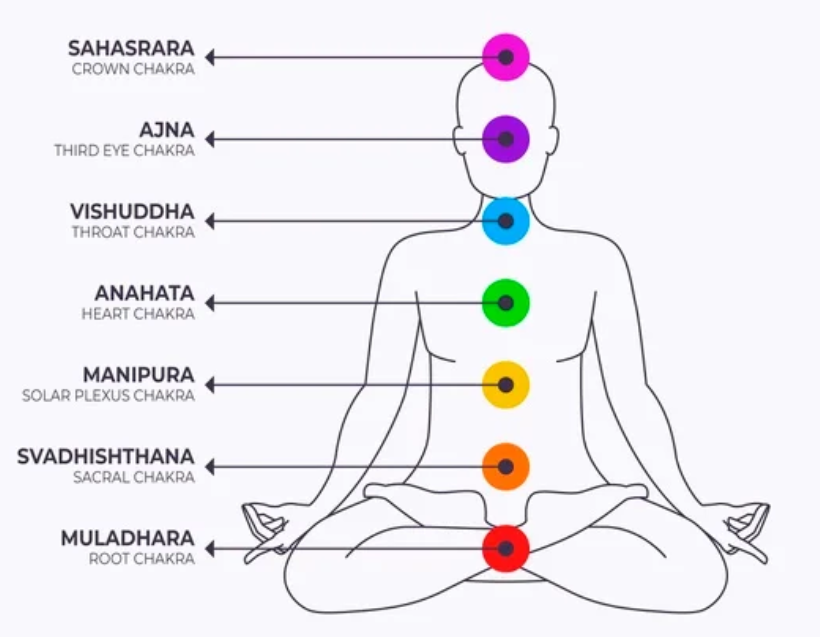
\includegraphics[width=0.7\linewidth,keepaspectratio]{ycb1_chakras}
				
		{\tiny (Ref: Raja Yoga Rishikesh)}	 
        \end{center}	

\end{frame}

%%%%%%%%%%%%%%%%%%%%%%%%%%%%%%%%%%%%%%%%%%%%%%%%%%%%%%%%%%
\begin{frame}[fragile]\frametitle{धातु Dhatus}
        \begin{center}
        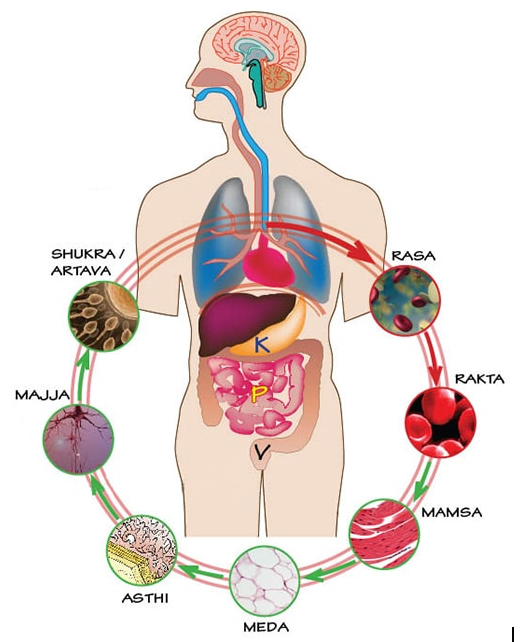
\includegraphics[width=0.5\linewidth,keepaspectratio]{ycb1_dhatus}
				
		{\tiny (Ref: Param Yoga)}	 
        \end{center}	

\end{frame}


%%%%%%%%%%%%%%%%%%%%%%%%%%%%%%%%%%%%%%%%%%%%%%%%%%%%%%%%%%%%%%%%%%%%%%%%%%%%%%%%%
\begin{frame}[fragile]\frametitle{}
\begin{center}
{\Large 1.5 Introduction to major schools of Yoga (ज्ञान Jnana, भक्ति  Bhakti, कर्म  Karma, पतञ्जलि  Patanjali, हठ Hatha)}
\end{center}
\end{frame}

%%%%%%%%%%%%%%%%%%%%%%%%%%%%%%%%%%%%%%%%%%%%%%%%%%%%%%%%%%
\begin{frame}[fragile]\frametitle{Philosophic Schools in Ancient India}
    \textbf{Types of Schools (दर्शन  Darshana):}
    \begin{itemize}
        \item \textbf{आस्तिक  दर्शन Astik Darshana} - Schools that follow the Vedas. (वेद प्रमाण ): न्याय (गौतम), वैशेषिक (कणाद), सांख्य (कपिल), मीमांसा (जैमिनी), योग(पतंजली), वेदांत (बादरायण)
        \item \textbf{नास्तिक  दर्शन  Nastik Darshana} - Schools that do not follow the authority of the Vedas नास्तिक : जैन (महावीर), बौद्ध , चार्वाक (बृहस्पती)
    \end{itemize}
	
    \textbf{Paths of Yoga:}
    \begin{itemize}
        \item \textbf{ ज्ञान योग Jnana Yoga}
        \item \textbf{भक्ती योग  Bhakti Yoga}
        \item \textbf{कर्म योग Karma Yoga}
        \item \textbf{राज योग Raja Yoga}
        \item \textbf{हठ योग Hatha Yoga}
        \item \textbf{मंत्र योग Mantra Yoga}
    \end{itemize}	
\end{frame}

% %%%%%%%%%%%%%%%%%%%%%%%%%%%%%%%%%%%%%%%%%%%%%%%%%%%%%%%%%%
% \begin{frame}[fragile]\frametitle{Astik Darshanas: Schools Following the Vedas}
    % \begin{tabular}{|l|l|}
    % \hline
    % \textbf{School Name} & \textbf{Founder} \\
    % \hline
    % \textbf{Nyaya} & Gautama Rishi \\
    % \hline
    % \textbf{Vaiseshika} & Kanada Rishi \\
    % \hline
    % \textbf{Sankhya} & Kapila Muni \\
    % \hline
    % \textbf{Yoga} & Patanjali Maharishi \\
    % \hline
    % \textbf{Purva Mimamsa} & Jaimini Rishi \\
    % \hline
    % \textbf{Uttara Mimamsa or Vedanta} & Vyasa Maharishi \\
    % \hline
    % \end{tabular}
% \end{frame}

% %%%%%%%%%%%%%%%%%%%%%%%%%%%%%%%%%%%%%%%%%%%%%%%%%%%%%%%%%%
% \begin{frame}[fragile]\frametitle{Nastik Darshanas: Schools Not Following the Vedas}
    % \begin{itemize}
        % \item \textbf{Charvaka}
        % \item \textbf{Buddhism}
        % \item \textbf{Jaina}
    % \end{itemize}
% \end{frame}

%%%%%%%%%%%%%%%%%%%%%%%%%%%%%%%%%%%%%%%%%%%%%%%%%%%%%%%%%%
\begin{frame}[fragile]\frametitle{ज्ञान योग  Jnana Yoga: Yoga of Wisdom}
    \textbf{Definition:} ज्ञान योग  Jnana Yoga is the path of self-realization through discerning the real from the unreal. It is a non-dualistic path that encourages the separation of the real from the illusory.

    
    \textbf{Three Stages of ज्ञान योग  Jnana Yoga Practice:}
    \begin{itemize}
        \item \textbf{श्रवण Sravana} - Listening or absorbing instructions
        \item \textbf{मनन Manana} - Reflection or contemplation involving reasoning
        \item \textbf{निधिध्यासना  Nidhidyasana} - Repeated meditation and implementation of convictions
    \end{itemize}

    \textbf{साधना चतुस्तय Sadhana Chatustaya:}
    \begin{itemize}
        \item \textbf{मनस Manas} - Mind
        \item \textbf{बुद्धि Buddhi} - Intellect
        \item \textbf{चित्त Chitta} - Consciousness
        \item \textbf{अहंकार Ahamkara} - Ego
    \end{itemize}
	
FOURFOLD साधना Sadhana of the student in the path of ज्ञान योग   Jnana Yoga consists of विवेक  Viveka, वैराग्य  Vairagya, षड्संपत  Shadshampat or sixfold virtues and मुमुक्षत्व   Mumukshutva or strong yearning for liberation. Sixfold path is विवेक  Viveka,वैराग्य  Vairagya, साम  Sama, दाम  Dama, उपरति  Uparati, तितिक्षा Titiksha, श्रद्धा Sraddha and समाधान Samadhana!
	
\end{frame}


%%%%%%%%%%%%%%%%%%%%%%%%%%%%%%%%%%%%%%%%%%%%%%%%%%%%%%%%%%%
\begin{frame}[fragile]\frametitle{भक्ति  योग Bhakti Yoga: Yoga of Devotion}
    \textbf{Definition:} Bhakti Yoga is the path of unconditional love for God, emphasizing devotion and the union of the lover (the yogi) with the beloved (the Divine).

    
    \textbf{Key Text:} नारद भक्ति सूत्र (Narada Bhakti Sutra) - Discusses the nature of भक्ति Bhakti and its connection to प्रेम Prema (divine love).

    
    \textbf{Techniques of भक्ति  योग Bhakti Yoga:}
    \begin{itemize}
        \item श्रवणं (shravan) : परिक्षित  parikshit
        \item कीर्तन (kirtan) : मिराबाई  mirabai, नारदमुनि narad muni (most important)
        \item स्मरण् smaran : प्रल्हाद  pralhad   
        \item पादसेवनम् पादुका paadsevan paduka: भरत bharat
        \item अर्चनम् (archanam) : एकलव्य ekalavya
        \item दास्य (dasya) : हनुमान hanuman
        \item सख्यं  (sakhya): sudama सुदामा
        \item आत्म निवेदनम् (aatma nvedan): bali raaja बाली राजा
    \end{itemize}

    
    \textbf{Types of भक्त  Bhaktas (Devotees) in भगवद्गीता  Bhagavad Gita:}
    \begin{itemize}
        \item \textbf{आर्त  Arta} - Distressed
        \item \textbf{अर्थार्थी Artharthee} - Desirer of wealth
        \item \textbf{जिज्ञासु Jidnasu} - Inquisitive
        \item \textbf{ज्ञानी Jnani} - Knowledgeable
		
    \end{itemize}
\end{frame}

%%%%%%%%%%%%%%%%%%%%%%%%%%%%%%%%%%%%%%%%%%%%%%%%%%%%%%%%%%%
\begin{frame}[fragile]\frametitle{कर्म योग  Karma Yoga: Yoga of Action}
          \begin{itemize}
	  \item \textbf{Definition:} Karma Yoga is the path of union through action. It is practiced by those with an outgoing or action-oriented nature. The key is to act selflessly, without personal gain or reward, and to offer the fruits of your actions to God.

 
	  \item \textbf{Core Principles of Karma Yoga (According to भगवद्गीता Bhagavad Gita):}
    \begin{enumerate}
        \item Work with a sense of duty.
        \item Work without intense attachment to the outcome.
        \item Do not let anxieties about results disturb your mind during the task.
        \item Accept both failure and success with equanimity.
    \end{enumerate}

	  \item  \textbf{Objective:} To sublimate the ego and achieve selfless devotion in all actions.
	      \end{itemize}

\end{frame}

%%%%%%%%%%%%%%%%%%%%%%%%%%%%%%%%%%%%%%%%%%%%%%%%%%%%%%%%%%%
\begin{frame}[fragile]\frametitle{राज  योग  Raja Yoga: The Royal Yoga}
    
      \begin{itemize}
	  \item \textbf{Definition:} Raja Yoga, meaning "royal" or "kingly" Yoga, is considered the culmination of all paths of Yoga. It represents the ultimate state of Self-realization.
	  \item  \textbf{Significance:} According to Swatmarama in the हठयोग प्रदीपिका (Hatha Yoga Pradipika), Hatha Yoga serves as a staircase leading to Raja Yoga. Raja Yoga may not refer to a specific form of Yoga but to the ultimate state of Self-realization.
	  \item \textbf{Objective:} To achieve cessation of mental modifications and restore the Real Self to its pristine purity, as emphasized by Patanjali.
		\item Focuses on the eight limbs of Yoga (\textit{अष्टान्ग Ashtanga Yoga}).
		\item Major text: \textit{Yoga Sutras of Patanjali}.
		\item Yogasutra/Rajayoga focuses on mental, Hathayoga focuses on physical
	  \end{itemize}
    
\end{frame}

%%%%%%%%%%%%%%%%%%%%%%%%%%%%%%%%%%%%%%%%%%%%%%%%%%%%%%%%%%%
\begin{frame}[fragile]\frametitle{हठ योग Hatha Yoga: The Physically Oriented Yoga}
    
\begin{itemize}
    \item Originates from Tantra, physically focused.
    \item Emphasizes purification (\textit{Shodhana Kriyas}/\textit{Shat Kriyas}, \textit{शोधन क्रिया}/\textit{षट्क्रिया}), unlike \textit{Yamas} (\textit{यम}) and \textit{Niyamas} (\textit{नियम}) of Ashtanga Yoga.
    \item Core texts:
    \begin{itemize}
        \item \textit{Hatha Yoga Pradipika} (\textit{हठयोगप्रदीपिका}) by Swatmarama
        \item \textit{Gheranda Samhita} (\textit{घेरंड संहिता}) by Sage Gheranda
        \item \textit{Goraksha Samhita} (\textit{गोरक्ष संहिता}) by Gorakshanath
        \item \textit{Shiv Samhita}, \textit{Yoga Rathnavali}, \textit{Yoga Taravali}, etc.
    \end{itemize}
    \item "Hatha" (\textit{हठ}) combines "ha" (\textit{ह} - sun, \textit{सूर्य}) and "tha" (\textit{ठ} - moon, \textit{चन्द्र}), uniting opposites.
    \item Sun: Heat, masculinity, effort; Moon: Coolness, femininity, surrender.
    \item Hatha Yoga balances opposites, fostering self-discovery.
    \item Misconception: "Hatha" is not stubbornness; it symbolizes union.
    \item \textit{Hatha Pradipika} (\textit{हठयोगप्रदीपिका}): Describes union of \textit{Pingala Nadi} (\textit{पिंगला नाड़ी} - sun) and \textit{Ida Nadi} (\textit{इडा नाड़ी} - moon), awakening \textit{Kundalini} (\textit{कुण्डलिनी}).
    \textit{Kundalini} travels through \textit{Sushumna Nadi} (\textit{सुषुम्ना नाड़ी}), crosses six \textit{Chakras} (\textit{चक्र}), unites with \textit{Brahman} (\textit{ब्रह्मन्}) at \textit{Sahasrara} (\textit{सहस्रार}).
    \item Union of \textit{Atma} (\textit{आत्मा}) and \textit{Paramatma} (\textit{परमात्मा}), leading to enlightenment.
    \item Goal: Control body and mind for spiritual growth.
\end{itemize}
    
\end{frame}


%%%%%%%%%%%%%%%%%%%%%%%%%%%%%%%%%%%%%%%%%%%%%%%%%%%%%%%%%%%
\begin{frame}[fragile]\frametitle{मंत्र योग Mantra Yoga: The Chanting oriented Yoga}
    
\begin{itemize}
    \item Mantra Yoga is the Yoga of sound.
    \item The word \textit{mantra मन्त्र} is derived from "man" (mind, मन) and "tra" (to protect,त्र).
    \item \textit{Mantra} means that which protects the mind .
    \item A mantra is a sacred utterance or sound charged with psycho-spiritual power.
    \item Mantra Yoga uses sound to achieve deep meditation and invoke specific states of consciousness.
    \item The power of the \textit{mantra} is realized through Mantra Yoga.
    \item The most important and recognized mantra is the sound of \textbf{Om} (\textit{ॐ}).
    \item \textbf{OM} is referred to as the \textit{mahamantra} (\textit{महामन्त्र}), the greatest of all mantras.
\end{itemize}
    
\end{frame}



%%%%%%%%%%%%%%%%%%%%%%%%%%%%%%%%%%%%%%%%%%%%%%%%%%%%%%%%%%%%%%%%%%%%%%%%%%%%%%%%%%
\begin{frame}[fragile]\frametitle{}
\begin{center}
{\Large 1.6 Introduction to Yoga practices for health and well being}
\end{center}
\end{frame}


%%%%%%%%%%%%%%%%%%%%%%%%%%%%%%%%%%%%%%%%%%%%%%%%%%%%%%%%%%%
\begin{frame}[fragile]\frametitle{Principles of Yoga Life}
योग्य जीवनाचे पाच सोपान 
      \begin{itemize}
		\item  व्यायाम: आसन 
		\item  श्वास: प्राणायाम 
		\item  आराम : शवासन 
		\item  अन्न : शाकाहारी 
		\item  सकारात्मक विचार आणि ध्यान 
	  \end{itemize}

\end{frame}
%%%%%%%%%%%%%%%%%%%%%%%%%%%%%%%%%%%%%%%%%%%%%%%%%%%%%%%%%%%
\begin{frame}[fragile]\frametitle{Health: Meaning and Definition}
    \textbf{World Health Organisation (WHO) Definition:}
    
        Health is defined as a state of complete physical, mental, social, and spiritual well-being and not merely the absence of disease or infirmity.
    

    
    \textbf{Sanskrit Definition:} 
    
        The Sanskrit word for health is स्वास्थ्य (Swasthya), derived from स्व (Swa) meaning "Self" and स्थ (Stha) meaning "abiding." Thus, Swasthya can be translated as "Abiding in one's own Self," reflecting the true nature of every being as सत्-चित्-आनन्द (Sat-Chit-Ananda) or being-Consciousness-Bliss.
    

    
    \textbf{Health according to Yoga:}
    \begin{itemize}
        \item Relaxed Muscles
        \item Loose joints to conserve energy
        \item Low metabolic rate
        \item Efficient utility of energy by the body
        \item Coordinated functioning of organ systems even under stress
    \end{itemize}
\end{frame}

%%%%%%%%%%%%%%%%%%%%%%%%%%%%%%%%%%%%%%%%%%%%%%%%%%%%%%%%%%%
\begin{frame}[fragile]\frametitle{Strength and Balance in Yoga}
    \textbf{Strength:}
    \begin{itemize}
        \item Yoga poses such as नौकासन (Naukasana), उत्कटासन (Utkatasana), and भुजंगासन (Bhujangasana) develop muscle strength similarly to traditional exercises like push-ups, lunges, or squats.
    \end{itemize}

    
    \textbf{Balance:}
    \begin{itemize}
        \item Balance is crucial for fitness and is often overlooked in traditional gym routines. 
        \item Yoga poses such as वृक्षासन (Vrikshasana or Tree Pose) teach practitioners to stay firm on one leg, enhancing overall balance and fitness for daily activities.
    \end{itemize}
\end{frame}

%%%%%%%%%%%%%%%%%%%%%%%%%%%%%%%%%%%%%%%%%%%%%%%%%%%%%%%%%%%
\begin{frame}[fragile]\frametitle{Joint Mobility and Yogic View of Health}
    \textbf{Joint Mobility:}
    \begin{itemize}
        \item Many Yoga poses require moving joints in ways different from linear activities like walking or running.
        \item This practice improves the overall range of motion and helps prevent injuries, reducing stiffness and pain.
    \end{itemize}

    
    \textbf{Yogic View of Health:}
    \begin{itemize}
        \item श्वेताश्वतर उपनिषद् (Shvetasvatara Upanishad): Health in Yoga is characterized by lightness of body, health, a desireless mind, clarity of complexion, a beautiful voice, an agreeable odor, and minimal excretions.
        \item Patanjali’s योग दर्शन (Yoga Darshan): Attributes of a perfect body include beauty, gracefulness, strength, and adamantine hardness. Deep concentration and mastery of सामान वायु (Samana Vayu) lead to radiant effulgence.
    \end{itemize}
\end{frame}

%%%%%%%%%%%%%%%%%%%%%%%%%%%%%%%%%%%%%%%%%%%%%%%%%%%%%%%%%%%
\begin{frame}[fragile]\frametitle{Mental and Emotional Well-being}
    \textbf{Mental Well-being:}
    \begin{itemize}
        \item Conscious process of calming the mind removes weaknesses.
        \item Builds willpower.
        \item Steadfastness becomes the core.
        \item Converts challenges into opportunities.
    \end{itemize}

    
    \textbf{Emotional Well-being:}
    \begin{itemize}
        \item Overcomes emotional conflicts, complexes, and turmoils.
        \item Sharpens and sensitizes emotions systematically.
    \end{itemize}
\end{frame}




%%%%%%%%%%%%%%%%%%%%%%%%%%%%%%%%%%%%%%%%%%%%%%%%%%%%%%%%%%%
\begin{frame}[fragile]\frametitle{Yoga Practices for Physical Health}

      \begin{itemize}
        \item \textit{Asanas} (आसन) (Postures) - Enhance flexibility, strength, and balance.
        \item \textit{Pranayama} (प्राणायाम) (Breath Control) - Improves lung capacity and energy flow.
        \item \textit{Shavasana} (शवासन) (Corpse Pose) - Promotes relaxation and recovery.
        \item \textit{Kriyas} (क्रियाः) (Cleansing Techniques) - Detoxify and purify the body.
        \item \textit{Bandhas} (बन्धाः) (Body Locks) - Support internal organ function and stability.
      \end{itemize}

\end{frame}

%%%%%%%%%%%%%%%%%%%%%%%%%%%%%%%%%%%%%%%%%%%%%%%%%%%%%%%%%%%
\begin{frame}[fragile]\frametitle{Yoga Practices for Mental Well-Being}

      \begin{itemize}
		\item \textit{Meditation} (Dhyana) - Reduces stress and enhances focus.
		\item \textit{Mindfulness} - Increases present-moment awareness and emotional stability.
		\item \textit{Pranayama} - Balances the nervous system and calms the mind.
		\item \textit{Mantra Chanting} - Provides mental clarity and emotional balance.
		\item \textit{Yoga Nidra} - Deep relaxation practice that improves sleep quality.
	  \end{itemize}

\end{frame}

%%%%%%%%%%%%%%%%%%%%%%%%%%%%%%%%%%%%%%%%%%%%%%%%%%%%%%%%%%%
\begin{frame}[fragile]\frametitle{Yoga Practices for Emotional Balance}

      \begin{itemize}
		\item \textit{Bhakti Yoga} - Cultivates emotional connection and devotion.
		\item \textit{Journaling} - Reflect on emotions and mental patterns.
		\item \textit{Gratitude Practice} - Enhances positive emotional states.
		\item \textit{Group Yoga Classes} - Builds community and support.
		\item \textit{Breath Awareness} - Helps in managing emotional responses.
	  \end{itemize}

\end{frame}

%%%%%%%%%%%%%%%%%%%%%%%%%%%%%%%%%%%%%%%%%%%%%%%%%%%%%%%%%%%
\begin{frame}[fragile]\frametitle{Yoga Practices for Overall Well-Being}

      \begin{itemize}
		\item \textit{Balanced Routine} - Integrate yoga into daily life for consistent benefits.
		\item \textit{Healthy Lifestyle Choices} - Complement yoga with proper nutrition and hydration.
		\item \textit{Holistic Approach} - Address physical, mental, and spiritual aspects.
		\item \textit{Regular Practice} - Ensure regular engagement for sustained well-being.
		\item \textit{Personalized Practice} - Adapt practices to individual needs and goals.
	  \end{itemize}

\end{frame}



%%%%%%%%%%%%%%%%%%%%%%%%%%%%%%%%%%%%%%%%%%%%%%%%%%%%%%%%%%%%%%%%%%%%%%%%%%%%%%%%%%
\begin{frame}[fragile]\frametitle{}
\begin{center}
{\Large 1.7 Introduction to \textit{Shatkarma} (षट्कर्म): meaning, purpose and their significance in \textit{Yoga Sadhana} (योग साधना)}
\end{center}
\end{frame}


%%%%%%%%%%%%%%%%%%%%%%%%%%%%%%%%%%%%%%%%%%%%%%%%%%%%%%%%%%%
\begin{frame}[fragile]\frametitle{Introduction to षटकर्म  Shatkarma}

      \begin{itemize}
		\item \textit{षटकर्म  Shatkarma} - Six purification techniques in Yoga.
		\item Aimed at cleansing the body and mind for enhanced spiritual practice.
		\item Prepares the practitioner for deeper practices like meditation and advanced postures.
		\item Integrates physical, mental, and energetic purification.
		\item Essential for holistic Yoga practice and overall health.
	  \end{itemize}

\end{frame}

%%%%%%%%%%%%%%%%%%%%%%%%%%%%%%%%%%%%%%%%%%%%%%%%%%%%%%%%%%%
\begin{frame}[fragile]\frametitle{Meaning and Purpose of षटकर्म Shatkarma}

      \begin{itemize}
		\item \textit{क्रिया Kriya} - Techniques to purify and balance the body.
		\item \textit{Purpose} - Remove toxins, enhance vitality, and stabilize the mind.
		\item \textit{Integration} - Facilitates deeper Yoga practices and spiritual growth.
		\item \textit{Holistic Cleansing} - Addresses physical, mental, and energetic levels.
		\item Essential for overcoming physical and mental obstructions.
	  \end{itemize}

\end{frame}

%%%%%%%%%%%%%%%%%%%%%%%%%%%%%%%%%%%%%%%%%%%%%%%%%%%%%%%%%%%
\begin{frame}[fragile]\frametitle{Significance of Shatkarma in Yoga Sadhana}

      \begin{itemize}
		\item \textit{Health Benefits} - Improves digestion, detoxifies, and boosts immunity.
		\item \textit{Mental Clarity} - Reduces stress and mental clutter.
		\item \textit{Energetic Balance} - Regulates the flow of vital energy (\textit{Prana}).
		\item \textit{Spiritual Preparation} - Prepares the practitioner for higher states of consciousness.
		\item \textit{Preventive Measures} - Aids in preventing diseases and imbalances.
	  \end{itemize}

\end{frame}

%%%%%%%%%%%%%%%%%%%%%%%%%%%%%%%%%%%%%%%%%%%%%%%%%%%%%%%%%%%
\begin{frame}[fragile]\frametitle{Overview of \textit{Shatkarma} (षट्कर्म) Techniques}

      \begin{itemize}
        \item \textit{Kapalabhati} (कपालभाती) - Skull Shining Breath for clearing nasal passages and energizing.
        \item \textit{Neti} (नेति) - Nasal cleansing with water or saline solution.
        \item \textit{Basti} (बस्ति) - Colonic cleansing to remove toxins from the intestines.
        \item \textit{Dhauti} (धौति) - Cleansing of the digestive tract through various methods.
        \item \textit{Trataka} (त्राटक) - Concentrated gazing to improve focus and cleanse the eyes.
        \item \textit{Nauli} (नौलि) - Abdominal massage to stimulate digestion and balance energy.
      \end{itemize}

\end{frame}



%%%%%%%%%%%%%%%%%%%%%%%%%%%%%%%%%%%%%%%%%%%%%%%%%%%%%%%%%%%%%%%%%%%%%%%%%%%%%%%%%%
\begin{frame}[fragile]\frametitle{}
\begin{center}
{\Large 1.8 Introduction to Yogic \textit{Sukshma Vyayama} (सूक्ष्म व्यायाम), \textit{Sthula Vyayama} (स्थूल व्यायाम) and \textit{Surya Namaskara} (सूर्य नमस्कार)}
\end{center}
\end{frame}


%%%%%%%%%%%%%%%%%%%%%%%%%%%%%%%%%%%%%%%%%%%%%%%%%%%%%%%%%%%
\begin{frame}[fragile]\frametitle{Introduction to Sukshma Vyayama}

      \begin{itemize}
		\item \textit{Sukshma Vyayama} - Subtle exercises for the body and mind.
		\item Focuses on gentle movements to prepare the body for more intensive practices.
		\item Enhances joint mobility and flexibility.
		\item Aids in the smooth functioning of internal organs.
		\item Ideal for warming up and increasing energy flow.
	  \end{itemize}

\end{frame}

%%%%%%%%%%%%%%%%%%%%%%%%%%%%%%%%%%%%%%%%%%%%%%%%%%%%%%%%%%%
\begin{frame}[fragile]\frametitle{Purpose and Benefits of Sukshma Vyayama}

      \begin{itemize}
		\item \textit{Improves Circulation} - Enhances blood flow to muscles and joints.
		\item \textit{Increases Flexibility} - Promotes flexibility in joints and muscles.
		\item \textit{Prepares Body} - Warms up the body before more rigorous exercises.
		\item \textit{Reduces Stiffness} - Alleviates joint and muscle stiffness.
		\item \textit{Calms Mind} - Prepares the mind for focused practice.
	  \end{itemize}

\end{frame}

%%%%%%%%%%%%%%%%%%%%%%%%%%%%%%%%%%%%%%%%%%%%%%%%%%%%%%%%%%%
\begin{frame}[fragile]\frametitle{Introduction to Sthula Vyayama}

      \begin{itemize}
		\item \textit{Sthula Vyayama} - Gross or physical exercises for the body.
		\item Includes more intense physical postures and movements.
		\item Aims to build strength, endurance, and overall physical fitness.
		\item Often used in combination with \textit{Sukshma Vyayama} for comprehensive practice.
		\item Focuses on major muscle groups and physical conditioning.
	  \end{itemize}

\end{frame}

%%%%%%%%%%%%%%%%%%%%%%%%%%%%%%%%%%%%%%%%%%%%%%%%%%%%%%%%%%%
\begin{frame}[fragile]\frametitle{Purpose and Benefits of Sthula Vyayama}

      \begin{itemize}
		\item \textit{Strength Building} - Develops muscle strength and endurance.
		\item \textit{Improves Posture} - Enhances overall body alignment and posture.
		\item \textit{Boosts Fitness} - Increases cardiovascular and physical fitness.
		\item \textit{Enhances Vitality} - Promotes general physical health and energy.
		\item \textit{Supports Weight Management} - Aids in maintaining a healthy weight.
	  \end{itemize}

\end{frame}

%%%%%%%%%%%%%%%%%%%%%%%%%%%%%%%%%%%%%%%%%%%%%%%%%%%%%%%%%%%
\begin{frame}[fragile]\frametitle{Introduction to \textit{Surya Namaskara} (सूर्य नमस्कार)}

      \begin{itemize}
        \item \textit{Surya Namaskara} (सूर्य नमस्कार) - Sun Salutation, a series of dynamic postures.
        \item Traditionally performed to honor the Sun and its energy.
        \item Consists of a sequence of 12 postures.
        \item Integrates movement, breath, and intention.
        \item Enhances overall physical and mental health.
      \end{itemize}

\end{frame}


%%%%%%%%%%%%%%%%%%%%%%%%%%%%%%%%%%%%%%%%%%%%%%%%%%%%%%%%%%%
\begin{frame}[fragile]\frametitle{Purpose and Benefits of Surya Namaskara}

      \begin{itemize}
		\item \textit{Improves Flexibility} - Stretches and tones the muscles.
		\item \textit{Boosts Circulation} - Enhances blood flow and energy levels.
		\item \textit{Increases Strength} - Builds core strength and endurance.
		\item \textit{Balances Mind} - Calms the mind and prepares for meditation.
		\item \textit{Energizes Body} - Invigorates and revitalizes overall health.
	  \end{itemize}

\end{frame}


%%%%%%%%%%%%%%%%%%%%%%%%%%%%%%%%%%%%%%%%%%%%%%%%%%%%%%%%%%%%%%%%%%%%%%%%%%%%%%%%%%
\begin{frame}[fragile]\frametitle{}
\begin{center}
{\Large 1.9 Introduction to \textit{Yogasana} (योगासन): meaning, principles, and their health benefits}
\end{center}
\end{frame}


%%%%%%%%%%%%%%%%%%%%%%%%%%%%%%%%%%%%%%%%%%%%%%%%%%%%%%%%%%%
\begin{frame}[fragile]\frametitle{Introduction to Yogasana}

      \begin{itemize}
		\item \textit{Yogasana} - Physical postures or poses in Yoga.
		\item Derived from the Sanskrit words \textit{Yoga} (union) and \textit{Asana} (seat or posture).
		\item Aims to harmonize body and mind through physical practice.
		\item Forms the foundation for many Yoga practices and techniques.
		\item Enhances physical and mental well-being.
	  \end{itemize}

\end{frame}

%%%%%%%%%%%%%%%%%%%%%%%%%%%%%%%%%%%%%%%%%%%%%%%%%%%%%%%%%%%
\begin{frame}[fragile]\frametitle{Principles of Yogasana}

      \begin{itemize}
		\item \textit{Alignment} - Proper positioning of body parts for effectiveness and safety.
		\item \textit{Breath Awareness} - Coordinating breath with movement to enhance practice.
		\item \textit{Balance} - Achieving physical and mental equilibrium in poses.
		\item \textit{Stability} - Maintaining a steady and comfortable posture.
		\item \textit{Mindfulness} - Being present and focused during practice.
	  \end{itemize}

\end{frame}

%%%%%%%%%%%%%%%%%%%%%%%%%%%%%%%%%%%%%%%%%%%%%%%%%%%%%%%%%%%
\begin{frame}[fragile]\frametitle{Health Benefits of Yogasana}

      \begin{itemize}
		\item \textit{Improves Flexibility} - Enhances range of motion in joints and muscles.
		\item \textit{Builds Strength} - Develops muscle strength and endurance.
		\item \textit{Enhances Posture} - Promotes proper alignment and balance.
		\item \textit{Boosts Circulation} - Improves blood flow and cardiovascular health.
		\item \textit{Reduces Stress} - Calms the mind and reduces anxiety levels.
		\item \textit{Improves Digestion} - Stimulates digestive organs and enhances metabolism.
		\item \textit{Enhances Mental Clarity} - Promotes focus, concentration, and mental well-being.
	  \end{itemize}

\end{frame}



%%%%%%%%%%%%%%%%%%%%%%%%%%%%%%%%%%%%%%%%%%%%%%%%%%%%%%%%%%%%%%%%%%%%%%%%%%%%%%%%%%
\begin{frame}[fragile]\frametitle{}
\begin{center}
{\Large 1.10 Introduction to \textit{Pranayama} (प्राणायाम) and \textit{Dhyana} (ध्यान) and their health benefits}
\end{center}
\end{frame}


%%%%%%%%%%%%%%%%%%%%%%%%%%%%%%%%%%%%%%%%%%%%%%%%%%%%%%%%%%%
\begin{frame}[fragile]\frametitle{Introduction to Pranayama}

      \begin{itemize}
		\item \textit{Pranayama} - The practice of breath control in Yoga.
		\item Derived from Sanskrit words \textit{Prana} (life force or breath) and \textit{Ayama} (control or extension).
		\item Aims to regulate and expand the breath to enhance life energy.
		\item Integrates breath with physical postures and meditation.
		\item Fundamental for balancing mind and body.
	  \end{itemize}

\end{frame}

%%%%%%%%%%%%%%%%%%%%%%%%%%%%%%%%%%%%%%%%%%%%%%%%%%%%%%%%%%%
\begin{frame}[fragile]\frametitle{Health Benefits of Pranayama}

      \begin{itemize}
		\item \textit{Improves Lung Capacity} - Enhances respiratory efficiency and endurance.
		\item \textit{Balances Nervous System} - Regulates stress and anxiety levels.
		\item \textit{Enhances Concentration} - Increases mental focus and clarity.
		\item \textit{Boosts Immunity} - Strengthens the immune system and overall vitality.
		\item \textit{Aids in Detoxification} - Promotes the removal of toxins from the body.
		\item \textit{Calms the Mind} - Reduces mental agitation and promotes relaxation.
		\item \textit{Regulates Emotions} - Helps in managing emotional responses and stability.
	  \end{itemize}

\end{frame}

%%%%%%%%%%%%%%%%%%%%%%%%%%%%%%%%%%%%%%%%%%%%%%%%%%%%%%%%%%%
\begin{frame}[fragile]\frametitle{Introduction to Dhyana}

      \begin{itemize}
		\item \textit{Dhyana} - Meditation or the practice of focused attention.
		\item Derived from Sanskrit meaning "profound contemplation" or "meditative absorption."
		• Aims to achieve a state of mental stillness and clarity.
		\item Involves sustained concentration and mindfulness.
		\item Integral for achieving higher states of consciousness and inner peace.
	  \end{itemize}

\end{frame}

%%%%%%%%%%%%%%%%%%%%%%%%%%%%%%%%%%%%%%%%%%%%%%%%%%%%%%%%%%%
\begin{frame}[fragile]\frametitle{Health Benefits of Dhyana}

      \begin{itemize}
		\item \textit{Reduces Stress} - Lowers cortisol levels and promotes relaxation.
		\item \textit{Enhances Emotional Well-Being} - Improves mood and emotional resilience.
		\item \textit{Improves Focus} - Increases attention span and cognitive function.
		\item \textit{Balances Blood Pressure} - Helps in maintaining healthy blood pressure levels.
		\item \textit{Promotes Inner Peace} - Fosters a sense of calm and tranquility.
		\item \textit{Aids in Self-Realization} - Encourages deeper self-awareness and understanding.
		\item \textit{Supports Mental Health} - Helps in managing anxiety, depression, and other mental health issues.
	  \end{itemize}

\end{frame}

